\documentclass[12pt,asmart]{report}
\usepackage[utf8]{inputenc}
\usepackage[margins]{trackchanges}
\usepackage{graphicx}
\usepackage{hyperref}
\usepackage{float}
\addeditor{Jake}
\graphicspath{ {images/} }

\usepackage{cite}

\usepackage[a4paper,width=150mm,top=22mm,bottom=25mm,bindingoffset=6mm]{geometry}


\usepackage{fancyhdr}
\pagestyle{fancy}


\title{\textbf{BackBlog Specification Document} 
\includegraphics{Newlogo.png}}
\author{\textbf{Nick Abegg (Writer), Josh Altmeyer, Jake Buhite (Editor), }\\\textbf{Tom Krusinski, Christian Totaro}}
\date{Fall 2023}


\begin{document}

\maketitle

\tableofcontents

\chapter{Introduction}
\section{Purpose}
\add[Jake]{Blah Blah}BackBlog is an app for social playlists, designed to enable the creation and sharing of collaborative movie and show playlists. Users can invite others to join in adding movies and shows to a shared playlist. This allows groups to easily keep track of movies and shows they are eager to watch together.
\section{Target User Group}
Our target user group is movie and TV show consumers. This is an extensive group with numerous subgroups, including two major categories: serious and casual consumers. The serious movie and show consumer watches a large quantity of media. They have an extensive list of movies and shows they want to watch which they constantly update. They likely have friends who also consume a similar amount of media. The casual movie and show consumer watches significantly fewer movies and shows. Due to not being able to watch movies and shows, they typically have a large backlog of movies and shows.
\section{Benefits to System Users}
There would be various benefits that an app like this would give a user.
\begin{itemize}
    \item Provides users with the ability to easily keep track of movies and shows they want to watch
    \item Collaboration on a log with friends
    \item Quickly search movies and shows and add them directly to the desired log
    \item View other's logs and movies and shows from their list to yours
    \item Easily rearrange logs if interest in a movie or show changes
\end{itemize}

\chapter{Design Information}
Creating the back end of BackBlog is an integral step in the development process. The system diagram will overview the general layout of the back-end interactions between a user and processes that accompany different user actions.
The user interface (UI) design of BackBlog was an iterative process that required constant revision, discussion, and evaluation. Much of the initial concepts and designs of the UI were based on the UI principles of conventionally popular streaming and playlist apps.
\section{Design Intro}
Creating the back end of BackBlog is an integral step in the development process. The system diagram will overview the general layout of the back-end interactions between a user and processes that accompany different user actions.
The user interface (UI) design of BackBlog was an iterative process that required constant revision, discussion, and evaluation. Much of the initial concepts and designs of the UI were based on the UI principles of conventionally popular streaming and playlist apps.
\section{System Diagram}
\begin{figure}[H]
    \centering
    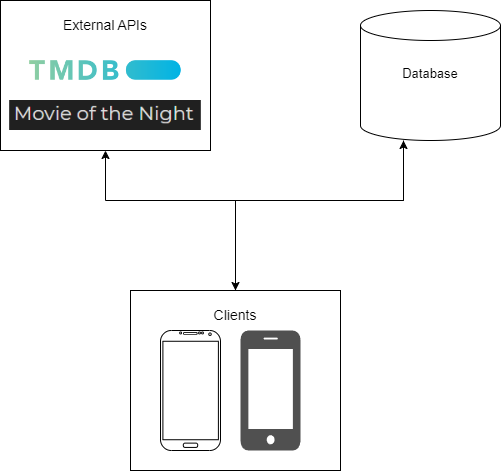
\includegraphics[width=1\linewidth]{systemdiagram.png}
    \caption{System Diagram}
    \label{SystemDiagram}
\end{figure}
The system diagram of BackBlog is shown above in figure \ref{SystemDiagram}. This showcases a very simple and abstract view of how our back-end will be set up for our app. Clients would be the users of the app who are searching for movies, creating logs, and adding friends. All of the movie-related information such as images, cast, genre, and movie name would all be queried from external APIs. Data such as creating logs, user info, and friends are stored on our own database shown on the top right. The logs would likely consist of movie ids that, when requested to be viewed by the user, are then utilized to query the database and display the movies from the log to the user.
\section{History of System Design}
As mentioned earlier, the BackBlog UI has gone through numerous iterations. 
\subsection{Early UI Mock-Up}
Below are two examples of an early mock-up of the UI and two examples of the final UI design.
\begin{figure}[H]
    \centering
    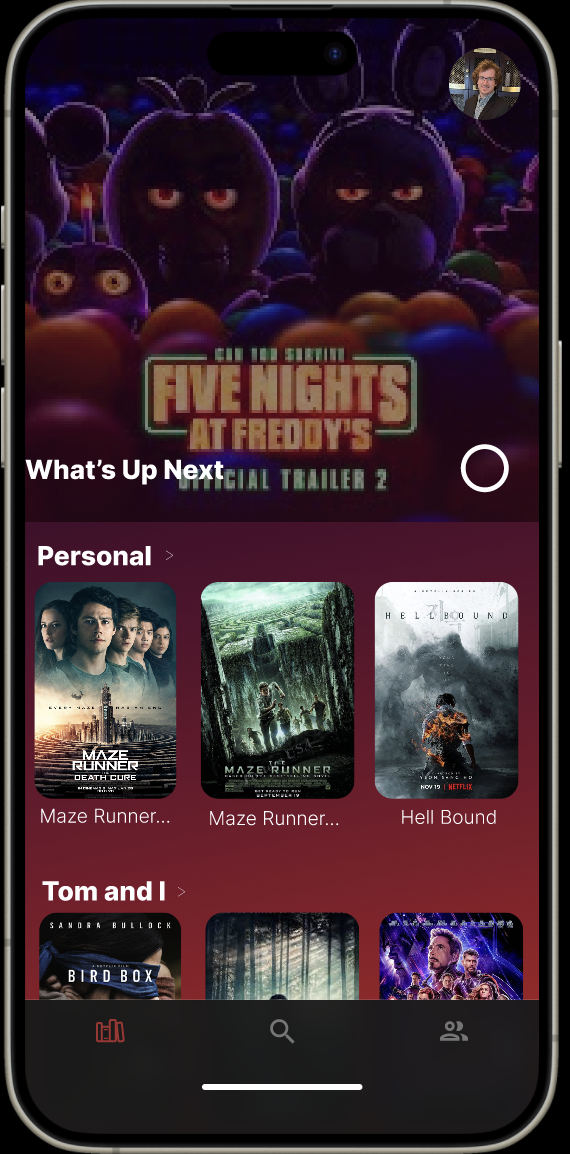
\includegraphics[width=.4\linewidth]{OldLandingPage.png}
    \caption{Early Landing Page UI}
    \label{OldLanding}
\end{figure}
Figure \ref{OldLanding} shows an early mock-up of our landing page. A "What's Up Next" section was added to be displayed as the first thing a user would see when opening up the app. Another notable design choice is the circle on the bottom right of this "What's Up Next" section which would allow the user to mark the movie as completed. There is also a profile selection at the top of the screen that would take the user to their profile. Lastly, There is a navigation menu to allow quick access to other parts of the app.
\begin{figure}[H]
    \centering
    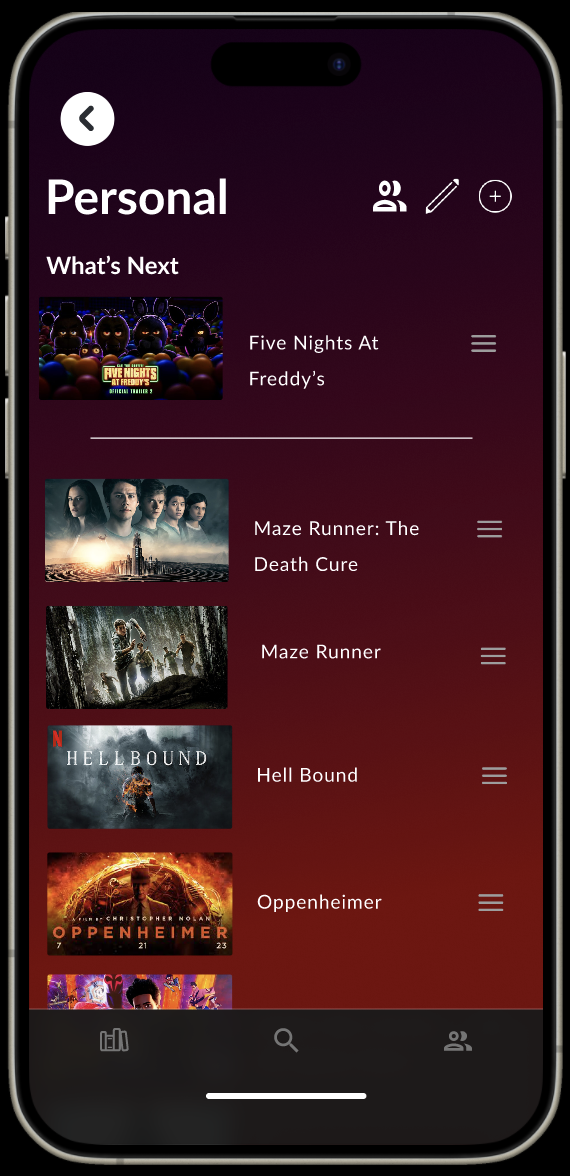
\includegraphics[width=.4\linewidth]{OldLogPage.png}
    \caption{Early Movie Log Page UI}
    \label{OldLog}
\end{figure}
Figure \ref{OldLog} showcases an early mock-up of a log page. This is the page that a user would see if they inspected a specific log they have either created or are collaborating on. The "What's Next" feature was also placed on this page. Additionally, the user has options to manage friends, edit details of the list and add to the log in the top right. Lastly, the user is able to quickly slide movies around in the list with the buttons to the right of the movies.
\subsection{Second UI Mock-Up}
However, due to user feedback and group discussion, small changes were made to better accommodate the interests and tastes of our users.
\begin{figure}[H]
    \centering
    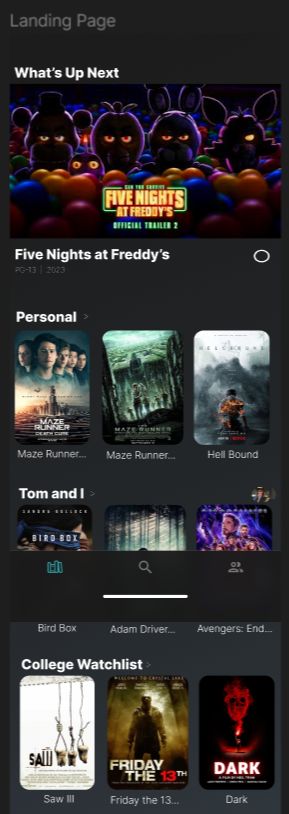
\includegraphics[width=0.4\linewidth]{LandingPage.png}
    \caption{Second Landing Page}
    \label{JoshLanding}
\end{figure}
Here in figure \ref{JoshLanding} you can see multiple changes were made to the final landing page. Notable changes are the removal of the profile button in the top right, shrinking the "What's Up Next" section, and moving the button to complete the "What's Up Next" movie outside below the section's area. Lastly, there is a profile picture shown on the bottom right next to the "Tom and I" movie log. These profiles show which users are collaborating on that backlog.
\begin{figure}[H]
    \centering
    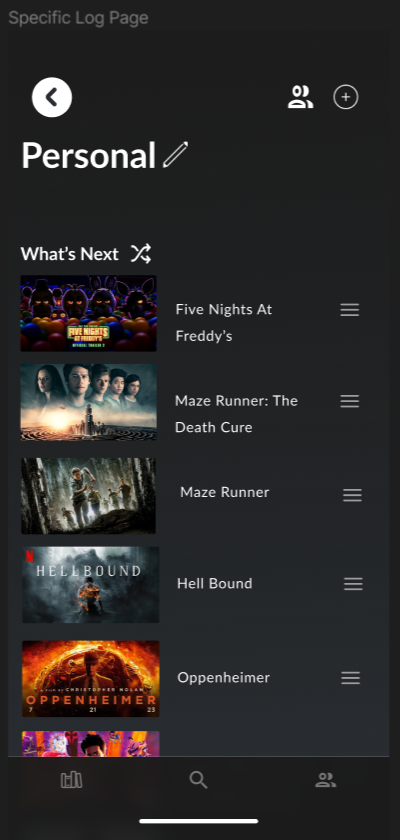
\includegraphics[width=0.4\linewidth]{LogPage.png}
    \caption{Second Log Page}
    \label{JoshLog}
\end{figure}
The log page was also modified and is shown in figure \ref{JoshLog} The line separating the "What's Next" and the rest of the list has been removed. Profile pictures showing which user added a movie to the list have been added. Many of the buttons for settings were also rearranged. The social and add movie buttons were moved higher up to the top right of the screen. The edit button for the log was moved next to the name. Lastly, a shuffle playlist button was added.

\subsection{Final UI Mock-Up}
Additionally, we had a separate fully interactive UI mock-up created. This one attempted to re-imagine the early mock-ups separately from the other mock-up designs.
\begin{figure}[H]
    \centering
    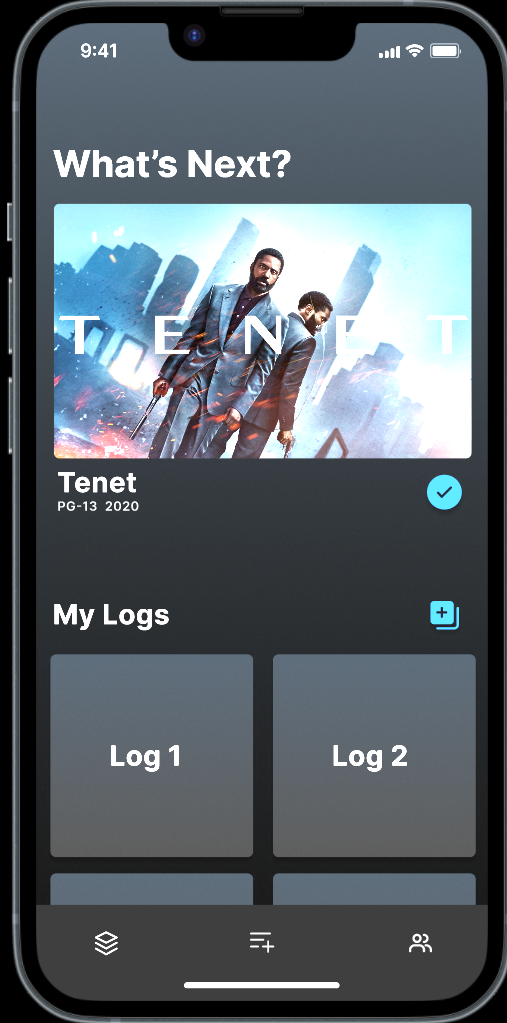
\includegraphics[width=.4\linewidth]{TomLanding.png}
    \caption{Final Landing Page}
    \label{TomLanding}
\end{figure}
Figure \ref{TomLanding} is of the alternate design. This showcases a different aesthetic to the early mock-up as well as the redesign mock-up. The "What's Up" section is still prominent but features alterations in style, font, text placement, and button placement. The "My Logs" section was redesigned to allow for easy selection of each log as well as quick access to create a new log with the plus button on the right.
\begin{figure}[H]
    \centering
    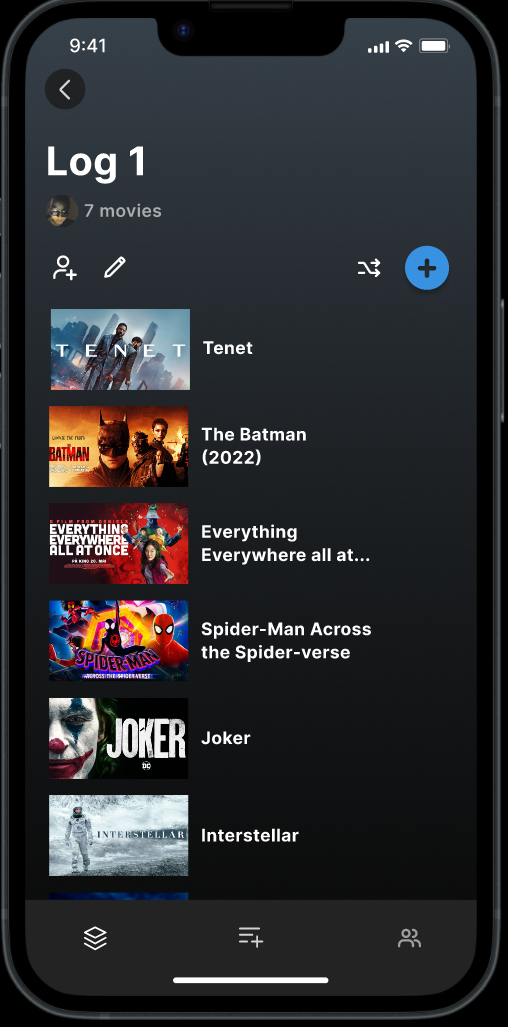
\includegraphics[width=0.4\linewidth]{TomLog.png}
    \caption{Final Log Page}
    \label{TomLog}
\end{figure}
Lastly, we redesigned the log screen as shown in figure \ref{TomLog}

We decided to utilize the alternate UI design and implement the most desirable features from the previous UI figure \ref{JoshLanding} \& \ref{JoshLog}.

The process of developing the UI required multiple interviews with different user groups and associated redesigns based on those user's feedback. Furthermore, the development of two separate UIs based on an early mock-up helped try different setups and designs on a variety of pages. Note that only the log and landing pages are showcased in this documentation but the designs were fully clickable with every page required in the final product.

\chapter{Design Evaluation}
\section{Design Heuristics}
\section{Results of User Testing}

\chapter{Ethical Assessment and IP}
\section{Ethical, Legal, Regulatory, and Social Issues}
In light of the inherent characteristics of a social media playlist, it is imperative to conscientiously address the ethical, moral, and legal challenges that the application may encounter.
\subsection{Ethical Considerations \& Social Issues}
Social media apps invite a multitude of ethical considerations \cite{Digital_Communications_Division_DCD2013-mf}. TABKA is obligated to consider all facets of these moral problems in designing our app and follow guidelines outlined in the Association for Computer Machinery Code of Ethics and Professional Conduct \cite{ACM_Code_2018_Task_Force_Executive_Committee_Don_Gotterbarn_Chair_Bo_Brinkman_Catherine_Flick_Michael_S_Kirkpatrick_Keith_Miller_Kate_Varansky_and_Marty_J_Wolf_Members_Eve_Anderson_Ron_Anderson_Amy_Bruckman_Karla_Carter_Michael_Davis_Penny_Duquenoy_Jeremy_Epstein_Kai_Kimppa_Lorraine_Kisselburgh_Shrawan_Kumar_Andrew_McGettrick_Natasa_Milic-Frayling_Denise_Oram_Simon_Rogerson_David_Shamma_Janice_Sipior_Eugene_Spafford_and_Les_Waguespack_undated-hy}.

\subsubsection{Data Protection}
Social media often rely on user-harvested data as the backbone of their financial model. Given that a large part of our app involves users deciding on what movies and shows to consume, there is a possibility for exploitation of this data for financial gain. Marketing and media companies would have a great interest in being able to track what users are interested in watching. Furthermore, the ability to influence which movies people consume would also be tantalizing. This is a tricky ethical situation as we have to weigh the financial gain we would make from selling user data to companies while maintaining user privacy. TABKA places the user's privacy and right to an advertiser-free environment above the financial gain that might be accumulated if we violate our user's privacy.

\subsubsection{Anonymity and Confidentiality}
Providing users with the ability to remain anonymous on our app is crucial to maintaining users right to privacy. TABKA will ensure that all information that directly relates to a user's identity, such as a user's name, will not be stored so as to ensure user anonymity is maintained. It is important to note that often information that might not be considered directly identifiable with a user's identity, can still result in users being identified. Through the combination of different information on a user, it may be possible to identify that user and compromise their integrity. TABKA will ensure that no directly identifiable information will be accessible or stored. However, TABKA cannot ensure that a user's anonymity can be maintained given the nature of social media and publicly available information.

\subsubsection{User Authenticity}
Users are allowed to freely create accounts that could impersonate someone without their consent. These impersonations could be damaging to a person's reputation and privacy \cite{Reichart_Smith2017-fe} \cite{Cox2014-sl}. TABKA will ensure that any harmful impersonation of person(s) without their consent will be swiftly removed. Repeated cases of impersonation will be properly escalated. TABKA will ensure that BackBlog will ensure account authenticity amongst its users.

\subsubsection{Minimizing Harm \& Protection of Minors}
It is important to consider the possibility of children using our app. Given that mature and adult content may be present on our app, minors might be exposed to content that could be considered inappropriate and harmful to their well-being. TABKA will require users to input their date of birth so as to confirm the age of the users. If a user is not over the age of 13, TABKA will prevent the user from creating an account on the app. Upon account creation, users will be prompted to consent to seeing mature or adult content.

\section{IP and Licensing \newline Considerations}
\begin{itemize}
    \item Social graph playlist that involves an automated method of identifying movies and songs that users are listening to, and then automatically crafting a playlist based on friend's activities. Similarity in the idea of a social playlist, however, differs in approach. BackBlog involves handpicked recommendations and playlist collaboration\cite{Murphy2010-gw}.
    \item Another patent found involves creating collaborative music playlists in real-time and sharing these playlists through social channels like social media. It is very similar to our concept of a social playlist but it is discussing specifically doing so with music. Not necessarily discussing the idea for movies \cite{Wheatley2011-pn}. It is unlikely this should cause any problems legally speaking in connection with our app.
    \item When it comes to designing BackBlog's UI, ensuring our layout is original and not infringing on a patented design is imperative to protecting BackBlog legally \cite{Phillips2019-ec}.
    \item If we do end up creating a recommendation system, avoiding a similar implementation is imperative to protecting BackBlog legally \cite{}
\end{itemize}
\subsection{Saint Vincent College IP Consideration}
Due to the fact that our app does not associate with Saint Vincent College (SVC) in any way, there should be no IP conflicts. Searching SVC's student portal yielded no IP-related issues based on the information publicly available on a variety of SVC documents.

\chapter{Assessment of Team Performance}

\chapter{Conclusion}


\nocite{*}
\bibliographystyle{IEEEannot}
\bibliography{references}

\end{document}